% Options for packages loaded elsewhere
% Options for packages loaded elsewhere
\PassOptionsToPackage{unicode}{hyperref}
\PassOptionsToPackage{hyphens}{url}
\PassOptionsToPackage{dvipsnames,svgnames,x11names}{xcolor}
%
\documentclass[
  letterpaper,
  DIV=11,
  numbers=noendperiod]{scrartcl}
\usepackage{xcolor}
\usepackage{amsmath,amssymb}
\setcounter{secnumdepth}{-\maxdimen} % remove section numbering
\usepackage{iftex}
\ifPDFTeX
  \usepackage[T1]{fontenc}
  \usepackage[utf8]{inputenc}
  \usepackage{textcomp} % provide euro and other symbols
\else % if luatex or xetex
  \usepackage{unicode-math} % this also loads fontspec
  \defaultfontfeatures{Scale=MatchLowercase}
  \defaultfontfeatures[\rmfamily]{Ligatures=TeX,Scale=1}
\fi
\usepackage{lmodern}
\ifPDFTeX\else
  % xetex/luatex font selection
\fi
% Use upquote if available, for straight quotes in verbatim environments
\IfFileExists{upquote.sty}{\usepackage{upquote}}{}
\IfFileExists{microtype.sty}{% use microtype if available
  \usepackage[]{microtype}
  \UseMicrotypeSet[protrusion]{basicmath} % disable protrusion for tt fonts
}{}
\makeatletter
\@ifundefined{KOMAClassName}{% if non-KOMA class
  \IfFileExists{parskip.sty}{%
    \usepackage{parskip}
  }{% else
    \setlength{\parindent}{0pt}
    \setlength{\parskip}{6pt plus 2pt minus 1pt}}
}{% if KOMA class
  \KOMAoptions{parskip=half}}
\makeatother
% Make \paragraph and \subparagraph free-standing
\makeatletter
\ifx\paragraph\undefined\else
  \let\oldparagraph\paragraph
  \renewcommand{\paragraph}{
    \@ifstar
      \xxxParagraphStar
      \xxxParagraphNoStar
  }
  \newcommand{\xxxParagraphStar}[1]{\oldparagraph*{#1}\mbox{}}
  \newcommand{\xxxParagraphNoStar}[1]{\oldparagraph{#1}\mbox{}}
\fi
\ifx\subparagraph\undefined\else
  \let\oldsubparagraph\subparagraph
  \renewcommand{\subparagraph}{
    \@ifstar
      \xxxSubParagraphStar
      \xxxSubParagraphNoStar
  }
  \newcommand{\xxxSubParagraphStar}[1]{\oldsubparagraph*{#1}\mbox{}}
  \newcommand{\xxxSubParagraphNoStar}[1]{\oldsubparagraph{#1}\mbox{}}
\fi
\makeatother

\usepackage{color}
\usepackage{fancyvrb}
\newcommand{\VerbBar}{|}
\newcommand{\VERB}{\Verb[commandchars=\\\{\}]}
\DefineVerbatimEnvironment{Highlighting}{Verbatim}{commandchars=\\\{\}}
% Add ',fontsize=\small' for more characters per line
\usepackage{framed}
\definecolor{shadecolor}{RGB}{241,243,245}
\newenvironment{Shaded}{\begin{snugshade}}{\end{snugshade}}
\newcommand{\AlertTok}[1]{\textcolor[rgb]{0.68,0.00,0.00}{#1}}
\newcommand{\AnnotationTok}[1]{\textcolor[rgb]{0.37,0.37,0.37}{#1}}
\newcommand{\AttributeTok}[1]{\textcolor[rgb]{0.40,0.45,0.13}{#1}}
\newcommand{\BaseNTok}[1]{\textcolor[rgb]{0.68,0.00,0.00}{#1}}
\newcommand{\BuiltInTok}[1]{\textcolor[rgb]{0.00,0.23,0.31}{#1}}
\newcommand{\CharTok}[1]{\textcolor[rgb]{0.13,0.47,0.30}{#1}}
\newcommand{\CommentTok}[1]{\textcolor[rgb]{0.37,0.37,0.37}{#1}}
\newcommand{\CommentVarTok}[1]{\textcolor[rgb]{0.37,0.37,0.37}{\textit{#1}}}
\newcommand{\ConstantTok}[1]{\textcolor[rgb]{0.56,0.35,0.01}{#1}}
\newcommand{\ControlFlowTok}[1]{\textcolor[rgb]{0.00,0.23,0.31}{\textbf{#1}}}
\newcommand{\DataTypeTok}[1]{\textcolor[rgb]{0.68,0.00,0.00}{#1}}
\newcommand{\DecValTok}[1]{\textcolor[rgb]{0.68,0.00,0.00}{#1}}
\newcommand{\DocumentationTok}[1]{\textcolor[rgb]{0.37,0.37,0.37}{\textit{#1}}}
\newcommand{\ErrorTok}[1]{\textcolor[rgb]{0.68,0.00,0.00}{#1}}
\newcommand{\ExtensionTok}[1]{\textcolor[rgb]{0.00,0.23,0.31}{#1}}
\newcommand{\FloatTok}[1]{\textcolor[rgb]{0.68,0.00,0.00}{#1}}
\newcommand{\FunctionTok}[1]{\textcolor[rgb]{0.28,0.35,0.67}{#1}}
\newcommand{\ImportTok}[1]{\textcolor[rgb]{0.00,0.46,0.62}{#1}}
\newcommand{\InformationTok}[1]{\textcolor[rgb]{0.37,0.37,0.37}{#1}}
\newcommand{\KeywordTok}[1]{\textcolor[rgb]{0.00,0.23,0.31}{\textbf{#1}}}
\newcommand{\NormalTok}[1]{\textcolor[rgb]{0.00,0.23,0.31}{#1}}
\newcommand{\OperatorTok}[1]{\textcolor[rgb]{0.37,0.37,0.37}{#1}}
\newcommand{\OtherTok}[1]{\textcolor[rgb]{0.00,0.23,0.31}{#1}}
\newcommand{\PreprocessorTok}[1]{\textcolor[rgb]{0.68,0.00,0.00}{#1}}
\newcommand{\RegionMarkerTok}[1]{\textcolor[rgb]{0.00,0.23,0.31}{#1}}
\newcommand{\SpecialCharTok}[1]{\textcolor[rgb]{0.37,0.37,0.37}{#1}}
\newcommand{\SpecialStringTok}[1]{\textcolor[rgb]{0.13,0.47,0.30}{#1}}
\newcommand{\StringTok}[1]{\textcolor[rgb]{0.13,0.47,0.30}{#1}}
\newcommand{\VariableTok}[1]{\textcolor[rgb]{0.07,0.07,0.07}{#1}}
\newcommand{\VerbatimStringTok}[1]{\textcolor[rgb]{0.13,0.47,0.30}{#1}}
\newcommand{\WarningTok}[1]{\textcolor[rgb]{0.37,0.37,0.37}{\textit{#1}}}

\usepackage{longtable,booktabs,array}
\usepackage{calc} % for calculating minipage widths
% Correct order of tables after \paragraph or \subparagraph
\usepackage{etoolbox}
\makeatletter
\patchcmd\longtable{\par}{\if@noskipsec\mbox{}\fi\par}{}{}
\makeatother
% Allow footnotes in longtable head/foot
\IfFileExists{footnotehyper.sty}{\usepackage{footnotehyper}}{\usepackage{footnote}}
\makesavenoteenv{longtable}
\usepackage{graphicx}
\makeatletter
\newsavebox\pandoc@box
\newcommand*\pandocbounded[1]{% scales image to fit in text height/width
  \sbox\pandoc@box{#1}%
  \Gscale@div\@tempa{\textheight}{\dimexpr\ht\pandoc@box+\dp\pandoc@box\relax}%
  \Gscale@div\@tempb{\linewidth}{\wd\pandoc@box}%
  \ifdim\@tempb\p@<\@tempa\p@\let\@tempa\@tempb\fi% select the smaller of both
  \ifdim\@tempa\p@<\p@\scalebox{\@tempa}{\usebox\pandoc@box}%
  \else\usebox{\pandoc@box}%
  \fi%
}
% Set default figure placement to htbp
\def\fps@figure{htbp}
\makeatother


% definitions for citeproc citations
\NewDocumentCommand\citeproctext{}{}
\NewDocumentCommand\citeproc{mm}{%
  \begingroup\def\citeproctext{#2}\cite{#1}\endgroup}
\makeatletter
 % allow citations to break across lines
 \let\@cite@ofmt\@firstofone
 % avoid brackets around text for \cite:
 \def\@biblabel#1{}
 \def\@cite#1#2{{#1\if@tempswa , #2\fi}}
\makeatother
\newlength{\cslhangindent}
\setlength{\cslhangindent}{1.5em}
\newlength{\csllabelwidth}
\setlength{\csllabelwidth}{3em}
\newenvironment{CSLReferences}[2] % #1 hanging-indent, #2 entry-spacing
 {\begin{list}{}{%
  \setlength{\itemindent}{0pt}
  \setlength{\leftmargin}{0pt}
  \setlength{\parsep}{0pt}
  % turn on hanging indent if param 1 is 1
  \ifodd #1
   \setlength{\leftmargin}{\cslhangindent}
   \setlength{\itemindent}{-1\cslhangindent}
  \fi
  % set entry spacing
  \setlength{\itemsep}{#2\baselineskip}}}
 {\end{list}}
\usepackage{calc}
\newcommand{\CSLBlock}[1]{\hfill\break\parbox[t]{\linewidth}{\strut\ignorespaces#1\strut}}
\newcommand{\CSLLeftMargin}[1]{\parbox[t]{\csllabelwidth}{\strut#1\strut}}
\newcommand{\CSLRightInline}[1]{\parbox[t]{\linewidth - \csllabelwidth}{\strut#1\strut}}
\newcommand{\CSLIndent}[1]{\hspace{\cslhangindent}#1}



\setlength{\emergencystretch}{3em} % prevent overfull lines

\providecommand{\tightlist}{%
  \setlength{\itemsep}{0pt}\setlength{\parskip}{0pt}}



 


\KOMAoption{captions}{tableheading}
\makeatletter
\@ifpackageloaded{caption}{}{\usepackage{caption}}
\AtBeginDocument{%
\ifdefined\contentsname
  \renewcommand*\contentsname{Table of contents}
\else
  \newcommand\contentsname{Table of contents}
\fi
\ifdefined\listfigurename
  \renewcommand*\listfigurename{List of Figures}
\else
  \newcommand\listfigurename{List of Figures}
\fi
\ifdefined\listtablename
  \renewcommand*\listtablename{List of Tables}
\else
  \newcommand\listtablename{List of Tables}
\fi
\ifdefined\figurename
  \renewcommand*\figurename{Figure}
\else
  \newcommand\figurename{Figure}
\fi
\ifdefined\tablename
  \renewcommand*\tablename{Table}
\else
  \newcommand\tablename{Table}
\fi
}
\@ifpackageloaded{float}{}{\usepackage{float}}
\floatstyle{ruled}
\@ifundefined{c@chapter}{\newfloat{codelisting}{h}{lop}}{\newfloat{codelisting}{h}{lop}[chapter]}
\floatname{codelisting}{Listing}
\newcommand*\listoflistings{\listof{codelisting}{List of Listings}}
\makeatother
\makeatletter
\makeatother
\makeatletter
\@ifpackageloaded{caption}{}{\usepackage{caption}}
\@ifpackageloaded{subcaption}{}{\usepackage{subcaption}}
\makeatother
\usepackage{bookmark}
\IfFileExists{xurl.sty}{\usepackage{xurl}}{} % add URL line breaks if available
\urlstyle{same}
\hypersetup{
  pdftitle={Deep dive into STANPUMP},
  pdfauthor={Jona JOACHIM},
  colorlinks=true,
  linkcolor={blue},
  filecolor={Maroon},
  citecolor={Blue},
  urlcolor={Blue},
  pdfcreator={LaTeX via pandoc}}


\title{Deep dive into STANPUMP}
\author{Jona JOACHIM}
\date{2025-08-19}
\begin{document}
\maketitle


\subsection{Pharmacometrics, TCI and
STANPUMP}\label{pharmacometrics-tci-and-stanpump}

Target controlled infusion (TCI) is a technique where the infusion of
drugs is controlled in real time by algorithms to achieve quickly and
safely, without overshoot, the desired concentration of drug in a
patients blood and / or at the effect site of the drug. This technique,
while not limited to anesthesia, has seen wide application only in the
perioperative setting where anesthesia related drugs are infused to
obtain a stable sedation when total intravenous anesthesia (TIVA) is
used.

TCI is based on pharmacometric models called PKPD models for
pharmacokinetic-pharmacodynamic models. These models describe the drug
distribution and metabolism through the body (pharmacokinetics) and the
effect of the drug on the body (pharmacodynamics). Most of the time, the
effect will be the level of sedation but this is not mandatory. From the
first uses of TCI in the 1980s\textsuperscript{1} to today, a lot of
effort has gone into the development of new PKPD models. These models
are now available for nearly every drug used for anesthesia. A lot of
literature is available on PKPD models and model design and a lot of
software is available to build and fit these models. The best known
software is NONMEM but numerous others are available, even open source
software such as nlmixr2\textsuperscript{2}.

Most PKPD models for anesthesia are compartmental models with 3
compartments. A1 is typically the amount of drug in the plasma.
Additionally, Ce is the concentration in the ``effect compartment''
which drives the drug effect.

However, in order to use new models, these models need to be integrated
in the TCI systems.

Currently, there are few TCI systems available. Most are proprietary and
closed source. Additionally, the algorithms used for TCI, which needs to
inverse PKPD models, are less well known. The only open source TCI
system I'm aware of is
\href{https://opentci.org/code/stanpump}{STANPUMP} from the 1990s.

In this blog post, I will take a deep dive into the STANPUMP source code
to try and understand the algorithms involved and see if I can implement
them in a modern fashion. The aim is to understand the algorithms and
have a minimal open source implementation from which to work.

\subsection{Mathematics}\label{mathematics}

PKPD models can be described by a set of ordinary differential equations
(ODE) with one equation per compartment. In anesthesia, most drugs
follow a 3-compartment model with can be mathematically described as
follows:

\pandocbounded{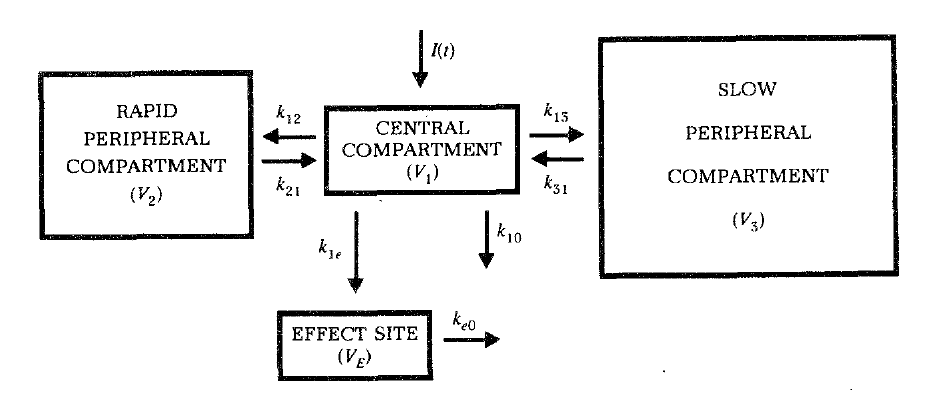
\includegraphics[keepaspectratio]{Screenshot_20250819_135400.png}}

\begin{equation}\phantomsection\label{eq-ode}{
\begin{equation}
\begin{aligned}
\frac{dA_1}{dt} & = A_2 k_{21} + A_3 k_{31} - A_1(k_{10} + k_{12} + k_{13}) + \text{Infusion} \\
\frac{dA_2}{dt} & = A_1 k_{12} - A_2 k_{21} \\
\frac{dA_3}{dt} & = A_1 k_{13} - A_3 k_{31} \\
\frac{dC_e}{dt} & = k_{e0}\left(\frac{A_1}{V_c} - C_e\right)
\end{aligned}
\end{equation}
}\end{equation}

\(A_n\) is the amount of drug in compartment \(n\), \(k_ij\) is the rate
constant which describes the speed with which the drug moves from
compartement \(i\) to compartment \(j\). This is not Fick's laws of
diffusion because diffusion is driven by concentration, not by drug
amount. It took me some time to understand that we are talking about the
drug amount, not the concentration. This was difficult to understand
especially since there is an exception for the effect site compartment
\(Ce\) where the rate constant \(k_e0\) drives directly concentration.
Once, the effect site compartment was treated as a regular compartment
(with \(k_14\) and \(k_41\) rate constants). However, nowadays it is
treated as a special compartment with zero volume and a single rate
constant \(k_e0\) (= \(k_41\)) and \(k_14\) is zero. Since the volume is
zero, no drug actually moves to the compartment and it is driven by
concentration.

If we leave aside the infusion term for one moment, we can write the
equations in matrix form as

\(\frac{dA}{dt} = S \cdot A^T\)

Where \(A\) is the vector

\begin{pmatrix} A_1 & A_2 & A_3 \end{pmatrix}

and S is the system matrix.

\[
\mathbf{S} = \begin{pmatrix}
-(k_{10} + k_{12} + k_{13}) & k_{21} & k_{31} \\
k_{12} & -k_{21} & 0 \\
k_{13} & 0 & -k_{31}
\end{pmatrix}
\]

This expression can be integrated to obtain the following closed form
expression:

\begin{equation}\phantomsection\label{eq-exponential}{
Cc(t) = A_1 e^{-\lambda_1 t} + A_2 e^{-\lambda_2 t} + A_3 e^{-\lambda_3 t}
}\end{equation}

or simply \(Cc = \sum_n A_n e^{-\lambda_n t}\)

For this, we need to calculate the exponential decay constants
\(\lambda\), which are the eigenvalues for the system.

However, this equation does not account for infusion, it describes the
clearance from plasma starting from an initial value \(A\).

If we want to solve the ODE system while taking into account the
infusion term \(J\), the equation becomes more
complicated\textsuperscript{3},\textsuperscript{4}. This equation
introduces coefficients \(c^p\) which are outlined below.

\(Cc = \sum_{n} A_n e^{-\lambda_n dt} + c^p_n J (1 - e^{-\lambda_n dt})\)

The equation can also be obtained for the effect site concentration:

\(Ce = \sum_{n} A_n e^{-\lambda_n dt} + c^e_n J (1 - e^{-\lambda_n dt})\)

In this case, the vector A contains a fourth term for the effect
compartment, \(k_e0\) is added as a fourth term to \(\lambda\) and
different coefficients \(c_e\) are used.

These formulas are valid for constant infusion rate \(J\). If the
infusion rate is changed, the solution can be calculated up to the last
value during the previous infusion rate and this solution can be used as
an initial state \(A\) in the new formula with new rate constant.

\subsubsection{Pharmacokinetic
Coefficient}\label{pharmacokinetic-coefficient}

This is the most frustrating part for me. I copied these coefficients
from STANPUMP but I don't know how to derive them mathematically.
Apparently, deriving them involves applying the Laplace transform to
Equation~\ref{eq-ode}, do some operations in the Laplace domain,
simplify the expression using partial fraction decomposition and apply
the inverse Laplace transform. However these maths are beyond what I
understand. I would be thrilled if somebody could explain to me how the
coefficients are derived.

\paragraph{Three Compartment Model}\label{three-compartment-model}

\[
\begin{equation}
\begin{aligned}
c^p_1 & = \frac{(k_{21} - \lambda_1)(k_{31} - \lambda_1)}{(\lambda_1 - \lambda_2)(\lambda_1 - \lambda_3) \cdot V_c \cdot \lambda_1}
\\
c^p_2 & = \frac{(k_{21} - \lambda_2)(k_{31} - \lambda_2)}{(\lambda_2 - \lambda_1)(\lambda_2 - \lambda_3) \cdot V_c \cdot \lambda_2}
\\
c^p_3 & = \frac{(k_{21} - \lambda_3)(k_{31} - \lambda_3)}{(\lambda_3 - \lambda_2)(\lambda_3 - \lambda_1) \cdot V_c \cdot \lambda_3}
\\
c^e_1 & = c^p_1 \cdot \frac{k_{e0}}{k_{e0} - \lambda_1}
\\
c^e_2 & = c^p_2 \cdot \frac{k_{e0}}{k_{e0} - \lambda_2}
\\
c^e_3 & = c^p_3 \cdot \frac{k_{e0}}{k_{e0} - \lambda_3}
\\
c^e_4 & = \frac{(k_{e0} - k_{21})(k_{e0} - k_{31})}{(\lambda_1 - k_{e0})(\lambda_2 - k_{e0})(\lambda_3 - k_{e0}) \cdot V_c}
\end{aligned}
\end{equation}
\]

\subsubsection{Two Compartment Model}\label{two-compartment-model}

\[
\begin{equation}
\begin{aligned}
c^p_1 & = \frac{k_{21} - \lambda_1}{(\lambda_2 - \lambda_1) \cdot V_c \cdot \lambda_1}
\\
c^p_2 & = \frac{k_{21} - \lambda_2}{(\lambda_1 - \lambda_2) \cdot V_c \cdot \lambda_2}
\\
c^e_1 & = c^p_1 \cdot \frac{k_{e0}}{k_{e0} - \lambda_1}
\\
c^e_2 & = c^p_2 \cdot \frac{k_{e0}}{k_{e0} - \lambda_2}
\\
c^e_3 & = \frac{k_{21} - k_{e0}}{(\lambda_1 - k_{e0})(\lambda_2 - k_{e0}) \cdot V_c}
\end{aligned}
\end{equation}
\]

\subsubsection{One Compartment Model}\label{one-compartment-model}

\[
\begin{equation}
\begin{aligned}
c_{p1} & = \frac{1}{\lambda_1 \cdot V_c}
\\
e_{p1} & = c_{p1} \cdot \frac{k_{e0}}{k_{e0} - \lambda_1}
\\
e_{p1} & = \frac{1}{(\lambda_1 - k_{e0}) \cdot V_c}
\end{aligned}
\end{equation}
\]

\subsection{Source code}\label{source-code}

The original source code for STANPUMP was written by Steven L. Shafer,
one of the fathers of TCI. Steven Shafer wanted this software to be open
source from the beginning which is a real gift for the community. Later,
Charles Minto created the Open TCI website, which collects models and
software related to PKPD and TCI. The latest version of STANPUMP is
available here: \url{https://opentci.org/code/stanpump}.

\subsubsection{16-bit real mode MSDOS}\label{bit-real-mode-msdos}

STANPUMP was written for the MSDOS operating system, running on x86
systems in ``real mode''. In real mode, program address physical memory
directly with a maximum of 1 MB adressable memory. There is no memory
protection and any memory location can be read and written by any
program. The program interacts directly with the hardware through
interrupts. This can for example be seen in the STANPUMP code which
interacts with the keyboard or renders text on the screen.

\begin{Shaded}
\begin{Highlighting}[]
\PreprocessorTok{\#define INT09   }\BaseNTok{0x0009}\PreprocessorTok{      }\CommentTok{/* Keyboard interrupt number           */}
\PreprocessorTok{\#define INT1B   }\BaseNTok{0x001B}\PreprocessorTok{      }\CommentTok{/* Ctrl{-}C interrupt number             */}
\PreprocessorTok{\#define INT23   }\BaseNTok{0x0023}\PreprocessorTok{      }\CommentTok{/* Ctrl{-}Break interrupt number         */}

\DataTypeTok{void}\NormalTok{ set\_keyboard}\OperatorTok{()}
    \OperatorTok{\{}
\NormalTok{       OldInt09 }\OperatorTok{=}\NormalTok{ \_dos\_getvect}\OperatorTok{(}\NormalTok{ INT09 }\OperatorTok{);}
\NormalTok{       OldInt1B }\OperatorTok{=}\NormalTok{ \_dos\_getvect}\OperatorTok{(}\NormalTok{ INT1B }\OperatorTok{);}
\NormalTok{       OldInt23 }\OperatorTok{=}\NormalTok{ \_dos\_getvect}\OperatorTok{(}\NormalTok{ INT23 }\OperatorTok{);}

\NormalTok{       KbdPtr }\OperatorTok{=}\NormalTok{ Int09}\OperatorTok{;}
\NormalTok{       \_dos\_setvect}\OperatorTok{(}\NormalTok{ INT09}\OperatorTok{,}\NormalTok{ KbdPtr }\OperatorTok{);}

\NormalTok{       BrkPtr }\OperatorTok{=}\NormalTok{ Int1B}\OperatorTok{;}
\NormalTok{       \_dos\_setvect}\OperatorTok{(}\NormalTok{ INT1B}\OperatorTok{,}\NormalTok{ BrkPtr}\OperatorTok{);}

\NormalTok{       BrkPtr }\OperatorTok{=}\NormalTok{ Int23}\OperatorTok{;}
\NormalTok{       \_dos\_setvect}\OperatorTok{(}\NormalTok{ INT23}\OperatorTok{,}\NormalTok{ BrkPtr }\OperatorTok{);}

\NormalTok{       KbdCtrl  }\OperatorTok{=} \OperatorTok{(}\NormalTok{ADDRESS}\OperatorTok{)}\NormalTok{ KBDFLAG}\OperatorTok{;}
\NormalTok{       keyboard\_reset }\OperatorTok{=} \DecValTok{1}\OperatorTok{;}
    \OperatorTok{\}}

\DataTypeTok{void}\NormalTok{ gotoxy}\OperatorTok{(}\NormalTok{x}\OperatorTok{,}\NormalTok{ y}\OperatorTok{)}
\DataTypeTok{int}\NormalTok{ x}\OperatorTok{,}\NormalTok{ y}\OperatorTok{;}
    \OperatorTok{\{}                   \CommentTok{/* gotoxy */}
\NormalTok{    REGS ir}\OperatorTok{,}\NormalTok{ or}\OperatorTok{;}
\NormalTok{    ir}\OperatorTok{.}\NormalTok{h}\OperatorTok{.}\NormalTok{dh }\OperatorTok{=}\NormalTok{ y}\OperatorTok{;}
\NormalTok{    ir}\OperatorTok{.}\NormalTok{h}\OperatorTok{.}\NormalTok{dl }\OperatorTok{=}\NormalTok{ x}\OperatorTok{;}
\NormalTok{    ir}\OperatorTok{.}\NormalTok{h}\OperatorTok{.}\NormalTok{ah }\OperatorTok{=} \DecValTok{2}\OperatorTok{;}
\NormalTok{    ir}\OperatorTok{.}\NormalTok{h}\OperatorTok{.}\NormalTok{bh }\OperatorTok{=} \DecValTok{0}\OperatorTok{;}
\NormalTok{    int86}\OperatorTok{(}\BaseNTok{0x10}\OperatorTok{,} \OperatorTok{\&}\NormalTok{ir}\OperatorTok{,} \OperatorTok{\&}\NormalTok{or}\OperatorTok{);}
    \OperatorTok{\}}                   \CommentTok{/* gotoxy */}
\end{Highlighting}
\end{Shaded}

\subsubsection{K\&R vs.~ANSI C}\label{kr-vs.-ansi-c}

STANPUMP is written in the now obsolete K\&R style which was published
in 1978 by Brian Kernighan and Dennis Ritchie.

This is mostly visible in the function prototypes, for example:

\begin{Shaded}
\begin{Highlighting}[]
\DataTypeTok{void}\NormalTok{ cube}\OperatorTok{(}\NormalTok{k10}\OperatorTok{,}\NormalTok{k12}\OperatorTok{,}\NormalTok{k21}\OperatorTok{,}\NormalTok{k13}\OperatorTok{,}\NormalTok{k31}\OperatorTok{,}\NormalTok{r}\OperatorTok{)}
\DataTypeTok{double}\NormalTok{ k10}\OperatorTok{,}\NormalTok{ k12}\OperatorTok{,}\NormalTok{ k21}\OperatorTok{,}\NormalTok{ k13}\OperatorTok{,}\NormalTok{ k31}\OperatorTok{;}
\DataTypeTok{double} \OperatorTok{*}\NormalTok{r}\OperatorTok{;}
    \OperatorTok{\{}                   \CommentTok{/* cube */}
    \CommentTok{/* function code */}
    \OperatorTok{\}}                   \CommentTok{/* cube */}
\end{Highlighting}
\end{Shaded}

This is the modern ANSI C equivalent of this prototype:

\begin{Shaded}
\begin{Highlighting}[]
\DataTypeTok{void}\NormalTok{ cube}\OperatorTok{(}\DataTypeTok{double}\NormalTok{ k10}\OperatorTok{,} \DataTypeTok{double}\NormalTok{ k12}\OperatorTok{,} \DataTypeTok{double}\NormalTok{ k21}\OperatorTok{,} \DataTypeTok{double}\NormalTok{ k13}\OperatorTok{,} \DataTypeTok{double}\NormalTok{ k31}\OperatorTok{,} \DataTypeTok{double} \OperatorTok{*}\NormalTok{r}\OperatorTok{);}
\end{Highlighting}
\end{Shaded}

\subsubsection{Memory allocations}\label{memory-allocations}

Memory was very constrained on the systems on which STANPUMP was meant
to run. No heap allocation is performed since this was unpredictable on
MSDOS systems. Instead, all variables were statically allocated and all
state was shared through global variables.

Global variable usage is frown upon nowadays because it makes it hard to
reason about the state of the program and follow where the state was
altered. It can also make the state unpredictable when multiple
functions can alter it in different ways.

Some very smart design choices were made in STANPUMP to soften memory
and CPU needs. It can be seen that the developers understood the
algorithms deeply and precalculated certain values to be able to reuse
them later.

One example is the introduction of ``unit disposition functions'' or
UDFs.

\begin{Shaded}
\begin{Highlighting}[]
\CommentTok{/* calculate udf, plasma concentration, for an infusion of 1/second */}
\NormalTok{p\_udf}\OperatorTok{[}\DecValTok{0}\OperatorTok{]} \OperatorTok{=} \DecValTok{0}\OperatorTok{;}
\ControlFlowTok{for} \OperatorTok{(}\NormalTok{i }\OperatorTok{=} \DecValTok{1}\OperatorTok{;}\NormalTok{  i }\OperatorTok{\textless{}} \DecValTok{199}\OperatorTok{;}\NormalTok{  i}\OperatorTok{++)}
    \OperatorTok{\{}
\NormalTok{    temp1 }\OperatorTok{=}\NormalTok{ temp1 }\OperatorTok{*}\NormalTok{ l1 }\OperatorTok{+}\NormalTok{ p\_coef}\OperatorTok{[}\DecValTok{1}\OperatorTok{]} \OperatorTok{*} \OperatorTok{(}\DecValTok{1} \OperatorTok{{-}}\NormalTok{ l1}\OperatorTok{);}
\NormalTok{    temp2 }\OperatorTok{=}\NormalTok{ temp2 }\OperatorTok{*}\NormalTok{ l2 }\OperatorTok{+}\NormalTok{ p\_coef}\OperatorTok{[}\DecValTok{2}\OperatorTok{]} \OperatorTok{*} \OperatorTok{(}\DecValTok{1} \OperatorTok{{-}}\NormalTok{ l2}\OperatorTok{);}
\NormalTok{    temp3 }\OperatorTok{=}\NormalTok{ temp3 }\OperatorTok{*}\NormalTok{ l3 }\OperatorTok{+}\NormalTok{ p\_coef}\OperatorTok{[}\DecValTok{3}\OperatorTok{]} \OperatorTok{*} \OperatorTok{(}\DecValTok{1} \OperatorTok{{-}}\NormalTok{ l3}\OperatorTok{);}
\NormalTok{    p\_udf}\OperatorTok{[}\NormalTok{i}\OperatorTok{]} \OperatorTok{=}\NormalTok{ temp1 }\OperatorTok{+}\NormalTok{ temp2 }\OperatorTok{+}\NormalTok{ temp3}\OperatorTok{;}
    \OperatorTok{\}}
\end{Highlighting}
\end{Shaded}

The UDFs serve as step response of the model and are calculated for
plasma concentration and effect site concentration. They represent the
response of the model for a contant infusion of 1 unit of drug per
second. This needs to be calculated once and is kept in memory. This
response vector can then later be scaled with the real infusion value.

\subsubsection{Calculation of
Eigenvalues}\label{calculation-of-eigenvalues}

STANPUMP uses closed form solutions of the PKPD differential functions
in order be improve efficiency of calculations. These closed form
solutions have been derived and published by the authors among
others\textsuperscript{3},\textsuperscript{4}.

In order to obtain these equations, the eigenvalues of the PKPD model
need to be calculated. In the early 1990s, there were probably no
mathematics libraries widely available to calculate eigenvalues, so the
developers had to calculate them manually. This is done in the CUBE.C
file.

First, the deteriminant of the system matrix is calculated and presented
in the form of a depressed cubic equation: x\^{}3 + px + q = 0.

Now, in the 1990s, there probably weren't any off the shelf solvers for
cubic equations in C available either, so the authors used the
trigonometric solutino by Girolamo Cardano from the 16th century to
solve this equation and derive the eigenvalues. Trigonometric functions
were part of the C standard library since 1978 and extended in 1989.

\begin{Shaded}
\begin{Highlighting}[]
\DataTypeTok{void}\NormalTok{ cube}\OperatorTok{(}\NormalTok{k10}\OperatorTok{,}\NormalTok{k12}\OperatorTok{,}\NormalTok{k21}\OperatorTok{,}\NormalTok{k13}\OperatorTok{,}\NormalTok{k31}\OperatorTok{,}\NormalTok{r}\OperatorTok{)}
\DataTypeTok{double}\NormalTok{ k10}\OperatorTok{,}\NormalTok{ k12}\OperatorTok{,}\NormalTok{ k21}\OperatorTok{,}\NormalTok{ k13}\OperatorTok{,}\NormalTok{ k31}\OperatorTok{;}
\DataTypeTok{double} \OperatorTok{*}\NormalTok{r}\OperatorTok{;}
    \OperatorTok{\{}                   \CommentTok{/* cube */}
    \DataTypeTok{double}\NormalTok{ a0}\OperatorTok{,}\NormalTok{ a1}\OperatorTok{,}\NormalTok{ a2}\OperatorTok{;}  \CommentTok{/* factors in cubic equation */}
    \DataTypeTok{double}\NormalTok{ p}\OperatorTok{,}\NormalTok{ q}\OperatorTok{;}        \CommentTok{/* factors in transformed equation */}
    \DataTypeTok{double}\NormalTok{ phi}\OperatorTok{;}         \CommentTok{/* used for root solving */}
    \DataTypeTok{double}\NormalTok{ r1}\OperatorTok{;}          \CommentTok{/* also used for root solving */}
    \DataTypeTok{double}\NormalTok{ toradian}\OperatorTok{;}    \CommentTok{/* mathematical conversion from degrees to radians */}

\NormalTok{    toradian }\OperatorTok{=}\NormalTok{ asin}\OperatorTok{(}\FloatTok{1.0}\OperatorTok{)} \OperatorTok{*} \FloatTok{2.0} \OperatorTok{/} \FloatTok{180.0}\OperatorTok{;} \CommentTok{/* pi/180 */}

    \ControlFlowTok{if} \OperatorTok{(}\NormalTok{k31 }\OperatorTok{\textgreater{}} \DecValTok{0}\OperatorTok{)}
        \OperatorTok{\{}
        \CommentTok{/* first take roots of X\^{}3 + a2X\^{}2 + a1X\^{}1 + a0 = 0 */}
        \CommentTok{/* where the coefficients are : */}
\NormalTok{        a0 }\OperatorTok{=}\NormalTok{ k10 }\OperatorTok{*}\NormalTok{ k21 }\OperatorTok{*}\NormalTok{ k31}\OperatorTok{;}
\NormalTok{        a1 }\OperatorTok{=}\NormalTok{ k10 }\OperatorTok{*}\NormalTok{ k31 }\OperatorTok{+}\NormalTok{ k21 }\OperatorTok{*}\NormalTok{ k31 }\OperatorTok{+}\NormalTok{ k21 }\OperatorTok{*}\NormalTok{ k13 }\OperatorTok{+}\NormalTok{ k10 }\OperatorTok{*}\NormalTok{ k21 }\OperatorTok{+}\NormalTok{ k31 }\OperatorTok{*}\NormalTok{ k12}\OperatorTok{;}
\NormalTok{        a2 }\OperatorTok{=}\NormalTok{ k10 }\OperatorTok{+}\NormalTok{ k12 }\OperatorTok{+}\NormalTok{ k13 }\OperatorTok{+}\NormalTok{ k21 }\OperatorTok{+}\NormalTok{ k31}\OperatorTok{;}

        \CommentTok{/* now transform to x\^{}3 + px + q = 0 */}
\NormalTok{        p }\OperatorTok{=}\NormalTok{ a1 }\OperatorTok{{-}} \OperatorTok{(}\NormalTok{a2 }\OperatorTok{*}\NormalTok{ a2 }\OperatorTok{/} \FloatTok{3.0}\OperatorTok{);}
\NormalTok{        q }\OperatorTok{=} \OperatorTok{(}\DecValTok{2} \OperatorTok{*}\NormalTok{ a2 }\OperatorTok{*}\NormalTok{ a2 }\OperatorTok{*}\NormalTok{ a2 }\OperatorTok{/} \FloatTok{27.0}\OperatorTok{)} \OperatorTok{{-}} \OperatorTok{(}\NormalTok{a1 }\OperatorTok{*}\NormalTok{ a2 }\OperatorTok{/} \FloatTok{3.0}\OperatorTok{)} \OperatorTok{+}\NormalTok{ a0}\OperatorTok{;}
\NormalTok{        r1 }\OperatorTok{=}\NormalTok{ sqrt}\OperatorTok{({-}(}\NormalTok{p }\OperatorTok{*}\NormalTok{ p }\OperatorTok{*}\NormalTok{ p}\OperatorTok{)} \OperatorTok{/} \FloatTok{27.0}\OperatorTok{);}
\NormalTok{        phi }\OperatorTok{=} \OperatorTok{({-}}\NormalTok{q }\OperatorTok{/} \FloatTok{2.0}\OperatorTok{)} \OperatorTok{/}\NormalTok{ r1}\OperatorTok{;}
        \ControlFlowTok{if} \OperatorTok{(}\NormalTok{phi }\OperatorTok{\textgreater{}} \DecValTok{1}\OperatorTok{)}
\NormalTok{            phi }\OperatorTok{=} \DecValTok{1}\OperatorTok{;}
        \ControlFlowTok{else} \ControlFlowTok{if} \OperatorTok{(}\NormalTok{phi }\OperatorTok{\textless{}} \OperatorTok{{-}}\DecValTok{1}\OperatorTok{)}
\NormalTok{            phi }\OperatorTok{=} \OperatorTok{{-}}\DecValTok{1}\OperatorTok{;}
\NormalTok{        phi }\OperatorTok{=} \OperatorTok{(}\NormalTok{acos}\OperatorTok{(}\NormalTok{phi}\OperatorTok{)} \OperatorTok{/} \FloatTok{3.0}\OperatorTok{);}
\NormalTok{        r1 }\OperatorTok{=} \FloatTok{2.0} \OperatorTok{*}\NormalTok{ exp}\OperatorTok{(}\NormalTok{log}\OperatorTok{(}\NormalTok{r1}\OperatorTok{)} \OperatorTok{/} \FloatTok{3.0}\OperatorTok{);}
\NormalTok{        r}\OperatorTok{[}\DecValTok{1}\OperatorTok{]} \OperatorTok{=} \OperatorTok{{-}(}\NormalTok{cos}\OperatorTok{(}\NormalTok{phi}\OperatorTok{)} \OperatorTok{*}\NormalTok{ r1 }\OperatorTok{{-}}\NormalTok{ a2 }\OperatorTok{/} \FloatTok{3.0}\OperatorTok{);}
\NormalTok{        r}\OperatorTok{[}\DecValTok{2}\OperatorTok{]} \OperatorTok{=} \OperatorTok{{-}(}\NormalTok{cos}\OperatorTok{(}\NormalTok{phi }\OperatorTok{+} \FloatTok{120.0} \OperatorTok{*}\NormalTok{ toradian}\OperatorTok{)} \OperatorTok{*}\NormalTok{ r1 }\OperatorTok{{-}}\NormalTok{ a2 }\OperatorTok{/} \FloatTok{3.0}\OperatorTok{);}
\NormalTok{        r}\OperatorTok{[}\DecValTok{3}\OperatorTok{]} \OperatorTok{=} \OperatorTok{{-}(}\NormalTok{cos}\OperatorTok{(}\NormalTok{phi }\OperatorTok{+} \FloatTok{240.0} \OperatorTok{*}\NormalTok{ toradian}\OperatorTok{)} \OperatorTok{*}\NormalTok{ r1 }\OperatorTok{{-}}\NormalTok{ a2 }\OperatorTok{/} \FloatTok{3.0}\OperatorTok{);}
        \OperatorTok{\}}
    \ControlFlowTok{else}
        \OperatorTok{\{}
        \ControlFlowTok{if} \OperatorTok{(}\NormalTok{k21 }\OperatorTok{\textgreater{}} \DecValTok{0}\OperatorTok{)}
            \OperatorTok{\{}
            \CommentTok{/* first take roots of X\^{}2 {-} a1X\^{}1 + a0 = 0 */}
            \CommentTok{/* where the coefficients are : */}
\NormalTok{            a0 }\OperatorTok{=}\NormalTok{ k10 }\OperatorTok{*}\NormalTok{ k21}\OperatorTok{;}
\NormalTok{            a1 }\OperatorTok{=} \OperatorTok{{-}(}\NormalTok{k10 }\OperatorTok{+}\NormalTok{ k12 }\OperatorTok{+}\NormalTok{ k21}\OperatorTok{);}
\NormalTok{            r}\OperatorTok{[}\DecValTok{1}\OperatorTok{]} \OperatorTok{=} \OperatorTok{({-}}\NormalTok{a1 }\OperatorTok{+}\NormalTok{ sqrt}\OperatorTok{(}\NormalTok{a1 }\OperatorTok{*}\NormalTok{ a1 }\OperatorTok{{-}} \DecValTok{4} \OperatorTok{*}\NormalTok{ a0}\OperatorTok{))} \OperatorTok{/} \DecValTok{2}\OperatorTok{;}
\NormalTok{            r}\OperatorTok{[}\DecValTok{2}\OperatorTok{]} \OperatorTok{=} \OperatorTok{({-}}\NormalTok{a1 }\OperatorTok{{-}}\NormalTok{ sqrt}\OperatorTok{(}\NormalTok{a1 }\OperatorTok{*}\NormalTok{ a1 }\OperatorTok{{-}} \DecValTok{4} \OperatorTok{*}\NormalTok{ a0}\OperatorTok{))} \OperatorTok{/} \DecValTok{2}\OperatorTok{;}
\NormalTok{            r}\OperatorTok{[}\DecValTok{3}\OperatorTok{]} \OperatorTok{=} \DecValTok{0}\OperatorTok{;}
            \OperatorTok{\}}
        \ControlFlowTok{else}
            \OperatorTok{\{}
            \CommentTok{/* one compartment model */}
\NormalTok{            r}\OperatorTok{[}\DecValTok{1}\OperatorTok{]} \OperatorTok{=}\NormalTok{ k10}\OperatorTok{;}
\NormalTok{            r}\OperatorTok{[}\DecValTok{2}\OperatorTok{]} \OperatorTok{=} \DecValTok{0}\OperatorTok{;}
\NormalTok{            r}\OperatorTok{[}\DecValTok{3}\OperatorTok{]} \OperatorTok{=} \DecValTok{0}\OperatorTok{;}
            \OperatorTok{\}}
        \OperatorTok{\}}

    \CommentTok{/* sort {-} nothing fancy is needed */}
    \ControlFlowTok{if} \OperatorTok{(}\NormalTok{r}\OperatorTok{[}\DecValTok{2}\OperatorTok{]} \OperatorTok{\textgreater{}}\NormalTok{ r}\OperatorTok{[}\DecValTok{1}\OperatorTok{])}
\NormalTok{        swap}\OperatorTok{(\&}\NormalTok{r}\OperatorTok{[}\DecValTok{2}\OperatorTok{],} \OperatorTok{\&}\NormalTok{r}\OperatorTok{[}\DecValTok{1}\OperatorTok{]);}
    \ControlFlowTok{if} \OperatorTok{(}\NormalTok{r}\OperatorTok{[}\DecValTok{3}\OperatorTok{]} \OperatorTok{\textgreater{}}\NormalTok{ r}\OperatorTok{[}\DecValTok{1}\OperatorTok{])}
\NormalTok{        swap}\OperatorTok{(\&}\NormalTok{r}\OperatorTok{[}\DecValTok{3}\OperatorTok{],} \OperatorTok{\&}\NormalTok{r}\OperatorTok{[}\DecValTok{1}\OperatorTok{]);}
    \ControlFlowTok{if} \OperatorTok{(}\NormalTok{r}\OperatorTok{[}\DecValTok{3}\OperatorTok{]} \OperatorTok{\textgreater{}}\NormalTok{ r}\OperatorTok{[}\DecValTok{2}\OperatorTok{])}
\NormalTok{        swap}\OperatorTok{(\&}\NormalTok{r}\OperatorTok{[}\DecValTok{3}\OperatorTok{],} \OperatorTok{\&}\NormalTok{r}\OperatorTok{[}\DecValTok{2}\OperatorTok{]);}
    \OperatorTok{\}}                   \CommentTok{/* cube */}
\end{Highlighting}
\end{Shaded}

\subsubsection{Core algorithm}\label{core-algorithm}

In order tu study the algorithm, I extracted the core functions and
their dependencies, converted them to ANSI C and implemented a minimal C
program to run the algorithm.

The source code for this project can be found here:
\url{https://framagit.org/jaj/ministan/-/tree/main/c}

I thought it was important to run the original STANPUMP code to serve as
a reference implementation. Small errors can be easily introduced when
an algorithm is re-implemented and small errors can be difficult to
detect.

The reference implementation of STANPUMP can serve as a control to test
if the output of our code is correct.

All global variables were moved into a struct named Config to serve as a
state variable.

\begin{Shaded}
\begin{Highlighting}[]
\CommentTok{/* cube.c */}
\DataTypeTok{void}\NormalTok{ cube}\OperatorTok{(}\DataTypeTok{double}\NormalTok{ k10}\OperatorTok{,} \DataTypeTok{double}\NormalTok{ k12}\OperatorTok{,} \DataTypeTok{double}\NormalTok{ k21}\OperatorTok{,} \DataTypeTok{double}\NormalTok{ k13}\OperatorTok{,} \DataTypeTok{double}\NormalTok{ k31}\OperatorTok{,}
          \DataTypeTok{double} \OperatorTok{*}\NormalTok{r}\OperatorTok{);}

\CommentTok{/* udfs.c */}
\DataTypeTok{void}\NormalTok{ calculate\_udfs}\OperatorTok{(}\NormalTok{Config }\OperatorTok{*}\NormalTok{cfg}\OperatorTok{);}

\CommentTok{/* virtual\_model.c */}
\DataTypeTok{double}\NormalTok{ virtual\_model}\OperatorTok{(}\NormalTok{Config }\OperatorTok{*}\NormalTok{cfg}\OperatorTok{,} \DataTypeTok{double}\NormalTok{ vm1}\OperatorTok{,} \DataTypeTok{double}\NormalTok{ vm2}\OperatorTok{,} \DataTypeTok{double}\NormalTok{ vm3}\OperatorTok{,}
                     \DataTypeTok{double}\NormalTok{ vm4}\OperatorTok{,} \DataTypeTok{int}\NormalTok{ t}\OperatorTok{,} \DataTypeTok{int}\NormalTok{ flag}\OperatorTok{);}

\CommentTok{/* find\_peak.c */}
\DataTypeTok{int}\NormalTok{ find\_peak}\OperatorTok{(}\NormalTok{Config }\OperatorTok{*}\NormalTok{cfg}\OperatorTok{,} \DataTypeTok{int}\NormalTok{ current\_time}\OperatorTok{,} \DataTypeTok{double}\NormalTok{ rate}\OperatorTok{,} \DataTypeTok{double}\NormalTok{ temp1e}\OperatorTok{,}
              \DataTypeTok{double}\NormalTok{ temp2e}\OperatorTok{,} \DataTypeTok{double}\NormalTok{ temp3e}\OperatorTok{,} \DataTypeTok{double}\NormalTok{ temp4e}\OperatorTok{);}

\CommentTok{/* model.c */}
\DataTypeTok{double}\NormalTok{ model}\OperatorTok{(}\NormalTok{Config }\OperatorTok{*}\NormalTok{cfg}\OperatorTok{,} \DataTypeTok{double}\NormalTok{ temp1}\OperatorTok{,} \DataTypeTok{double}\NormalTok{ temp2}\OperatorTok{,} \DataTypeTok{double}\NormalTok{ temp3}\OperatorTok{,}
             \DataTypeTok{double}\NormalTok{ temp1e}\OperatorTok{,} \DataTypeTok{double}\NormalTok{ temp2e}\OperatorTok{,} \DataTypeTok{double}\NormalTok{ temp3e}\OperatorTok{,} \DataTypeTok{double}\NormalTok{ temp4e}\OperatorTok{,}
             \DataTypeTok{double}\NormalTok{ desired}\OperatorTok{);}
\end{Highlighting}
\end{Shaded}

The cube() function was already discussed above. It calculates
eigenvalues of the PK system which are widely used later in the code.

The calculate\_udfs() function calculates the ``unit disposition
functions'' (UDF). A 10 second infusion is simulated at constant (unit)
rate. Then the model is run until the model is run without infusion to
see when the concentration peaks (peak\_time). The peak\_time (also
called time to peak effect TTPE) is a caracteristic of the model. It is
used later in the model() function. The calculate\_udfs() function also
calculates the \(c^p\) and \(c^e\) coefficients.

The virtual\_model() function runs the model without infusion rate for a
specified time. This is useful to estimate where the concentrations are
heading and to evaluate how rate needs to be adjusted.

find\_peak() is a hill climbing algorithm to find out when concentration
will peak given the current infusion rate.

The model() function is the main function of the algorithm. It
orchestrates the other functions to find the optimal infusion rate for
the given target.

\subsection{Reimplementation in
Python}\label{reimplementation-in-python}

A lot of deep knowledge of TCI algorithms and programming skills went
into STANPUMP. The authors derived part of the mathematics themselves to
improve performance and used coding skills which made it possible to run
the algorithms in real time on very rudementary hardware. The software
has seen 10+ years of clinical usage and its algorithms are battle
tested.

In order to experiment with the code and run it with my own models, I
decided to reimplement the code in Python. First I did a (1:1
translation){[}https://framagit.org/jaj/ministan/-/blob/main/python/ministan.py{]}
of the C code and then I gradually replaced some parts with modern
idioms such as array programming with NumPy\textsuperscript{5}.

For example, the calculation of the eigenvalues is straightforward with
NumPy: `

\begin{Shaded}
\begin{Highlighting}[]
\ImportTok{import}\NormalTok{ numpy }\ImportTok{as}\NormalTok{ np}
\NormalTok{A }\OperatorTok{=}\NormalTok{ [}
\NormalTok{    [}\OperatorTok{{-}}\NormalTok{(k10 }\OperatorTok{+}\NormalTok{ k12 }\OperatorTok{+}\NormalTok{ k13), k21, k31],}
\NormalTok{    [k12, }\OperatorTok{{-}}\NormalTok{k21, }\DecValTok{0}\NormalTok{],}
\NormalTok{    [k13, }\DecValTok{0}\NormalTok{, }\OperatorTok{{-}}\NormalTok{k31],}
\NormalTok{]}
\NormalTok{lambdas }\OperatorTok{=}\NormalTok{ np.linalg.eigvals(A)}
\end{Highlighting}
\end{Shaded}

Probably some algorithms could be replaced by highly optimized functions
from the SciPy library\textsuperscript{6}, such as the hill climbing
algorithm in find\_peaks(). There is still work to be done in this
space.

The current version of the code can be found here:
\url{https://framagit.org/jaj/ministan/-/blob/main/python/tci.py}

Here is an example code of a simulation of the Gepts Sufentanil
model\textsuperscript{7}:

https://framagit.org/jaj/ministan/-/blob/main/python/sim\_gepts.py

The code calculates the rates for 3 different effect site targets and
calculates the plasma and effect site concentrations obtained with the
given rate. In addition to the closed form solutions, the code also
calculates the results directly from the ODEs to validate the result
using an independent calculation.

\pandocbounded{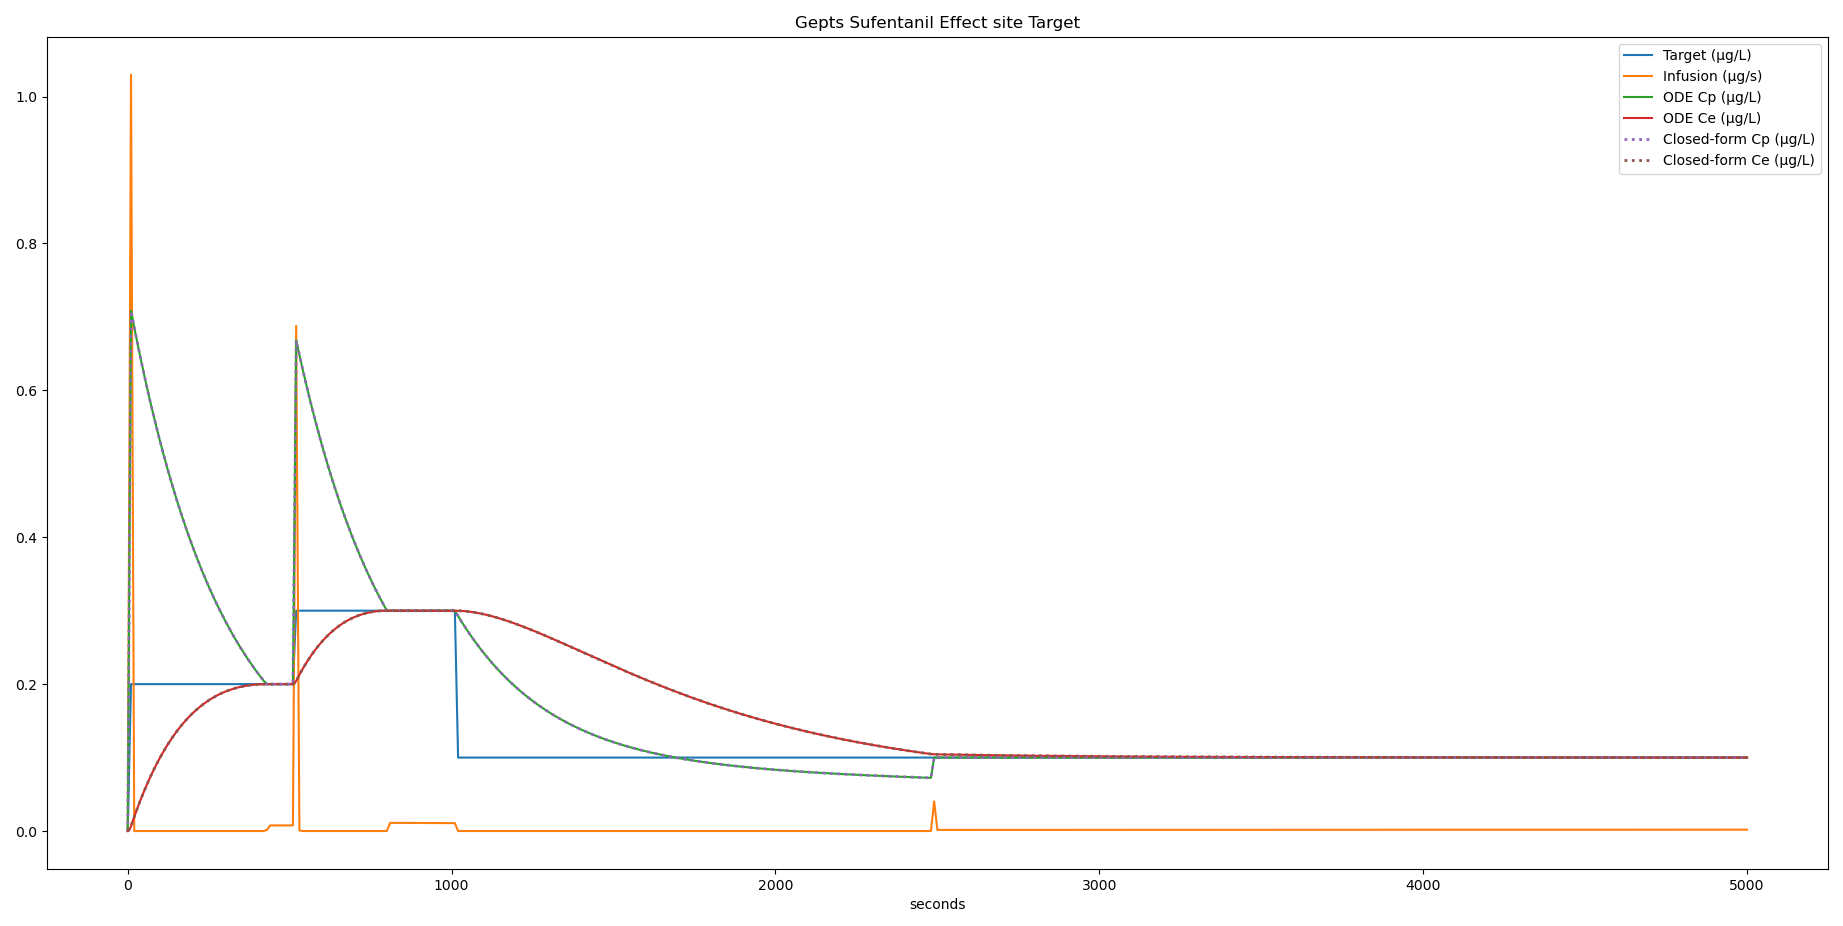
\includegraphics[keepaspectratio]{Figure_1.png}}

The code could be coupled to a syringe pump control library such as
InfuPy\textsuperscript{8} to drive syringe pumps with the calculated
rates. Of course this can only be used for research purposes and under
no circumstances on real patients. See
\url{https://www.demed.be/Rugloop\%20&\%20TCI\%20news.htm\#Background}
for more information on this topic.

\subsection{Emulation}\label{emulation}

\subsection{References}\label{references}

\phantomsection\label{refs}
\begin{CSLReferences}{0}{1}
\bibitem[\citeproctext]{ref-struys_history_2016}
\CSLLeftMargin{1. }%
\CSLRightInline{Struys MMRF, De Smet T, Glen J(Iain)B, Vereecke HEM,
Absalom AR, Schnider TW. The {History} of {Target}-{Controlled}
{Infusion}. \emph{Anesthesia \& Analgesia} {[}Internet{]} 2016 {[}cited
2025 Aug 19{]}; \textbf{122}: 56--69 Available from:
\url{https://journals.lww.com/00000539-201601000-00015}}

\bibitem[\citeproctext]{ref-nlmixr}
\CSLLeftMargin{2. }%
\CSLRightInline{Fidler M, Wilkins J, Hooijmaijers R, et al. Nonlinear
mixed-effects model development and simulation using nlmixr and related
r open-source packages. \emph{CPT: Pharmacometrics \& Systems
Pharmacology} {[}Internet{]} Hoboken: John Wiley; Sons Inc.; 2019;
\textbf{8}: 621--33 Available from:
\url{https://doi.org/10.1002/psp4.12445}}

\bibitem[\citeproctext]{ref-shafer_algorithms_1992}
\CSLLeftMargin{3. }%
\CSLRightInline{Shafer SL, Gregg KM. Algorithms to rapidly achieve and
maintain stable drug concentrations at the site of drug effect with a
computer-controlled infusion pump. \emph{Journal of Pharmacokinetics and
Biopharmaceutics} {[}Internet{]} 1992 {[}cited 2025 Aug 19{]};
\textbf{20}: 147--69 Available from:
\url{http://link.springer.com/10.1007/BF01070999}}

\bibitem[\citeproctext]{ref-bailey_simple_1991}
\CSLLeftMargin{4. }%
\CSLRightInline{Bailey JM, Shafer SL.
\href{https://doi.org/10.1109/10.81576}{A simple analytical solution to
the three-compartment pharmacokinetic model suitable for
computer-controlled infusion pumps}. \emph{IEEE transactions on
bio-medical engineering} 1991; \textbf{38}: 522--5 }

\bibitem[\citeproctext]{ref-harris2020array}
\CSLLeftMargin{5. }%
\CSLRightInline{Harris CR, Millman KJ, Walt SJ van der, et al. Array
programming with {NumPy}. \emph{Nature} {[}Internet{]} Springer Science;
Business Media {LLC}; 2020; \textbf{585}: 357--62 Available from:
\url{https://doi.org/10.1038/s41586-020-2649-2}}

\bibitem[\citeproctext]{ref-2020SciPy-NMeth}
\CSLLeftMargin{6. }%
\CSLRightInline{Virtanen P, Gommers R, Oliphant TE, et al.
\href{https://doi.org/10.1038/s41592-019-0686-2}{{{SciPy} 1.0:
Fundamental Algorithms for Scientific Computing in Python}}.
\emph{Nature Methods} 2020; \textbf{17}: 261--72 }

\bibitem[\citeproctext]{ref-gepts_linearity_1995}
\CSLLeftMargin{7. }%
\CSLRightInline{Gepts E, Shafer SL, Camu F, et al. Linearity of
{Pharmacokinetics} and {Model} {Estimation} of {Sufentanil}.
\emph{Anesthesiology} {[}Internet{]} 1995 {[}cited 2025 Aug 23{]};
\textbf{83}: 1194--204 Available from:
\url{https://journals.lww.com/00000542-199512000-00010}}

\bibitem[\citeproctext]{ref-joachim_jona_infupy_2021}
\CSLLeftMargin{8. }%
\CSLRightInline{Joachim J. {InfuPy} {[}Internet{]}. Zenodo; 2021
{[}cited 2021 Aug 16{]}. Available from:
\url{https://zenodo.org/record/5208192}}

\end{CSLReferences}




\end{document}
